V experimentálnej časti sme sa venovali porovaniu prístupov k odhadu parametrov a porovnaniu dvoch optimalizačných metód -- simplexovej (Nelder--Mead) metóde a metóde Luus--Jaakola. Dáta boli vygenerované modelom 
% RP: data boli vygenerovane simulaciou modelu, nie ``vygenerované modelom ''
s inhibíciou pri viacerých skokových zmenách v rýchlosti riedenia $D = $ (0.2, 0.3, 0.4 a 0.5\unitfrac{1}{\hour}) v čase $t = $ 50\unit{\hour} a ich časový priebeh je zobrazený na Obr. \ref{fig:1}. Parametre modelu boli nastavené podobne ako je uvedené v Tabuľke \ref{tab: 3} s rozdielom v maximálnej špecifickej rýchlosti rastu s hodnotou $\mu_{m} = $ 0.954\unitfrac{1}{\hour}. Odhad parametrov sme robili vzhľadom na Monod model, kvôli vyššie uvedeným skutočnostiam. 

Najväčším problémom pri odhade parametrov na základe aproximácie derivácie je šum merania. Diferencia takéhoto signálu vedie k strate údajov z dynamiky systému. Preto je potrebné takýto zašumený signál najskôr spracovať napr. filtráciou. Ďalším faktom je, že meranie koncentrácie biomasy má omnoho väčšiu fluktuáciu ako samotné meranie koncentrácie substrátu, čo vedie k väčším nepresnostiam. V praxi by bolo nutné zabezpečiť identifikáciu živých organizmov od mŕtvych, ak by sme chceli robiť odhad takýmto prístupom. Na Obr. \ref{fig:8} môžeme vidieť výsledok odhadu parametrov na základe aporximácie
% Rp: spell check ``aporximácie''
derivácie. Môžeme si všimnúť, že takýto prístup k odhadu parametrov kladie dôraz skôr na dynamiku systému ako na samotné ustálené stavy.

\begin{figure}
	\centering
	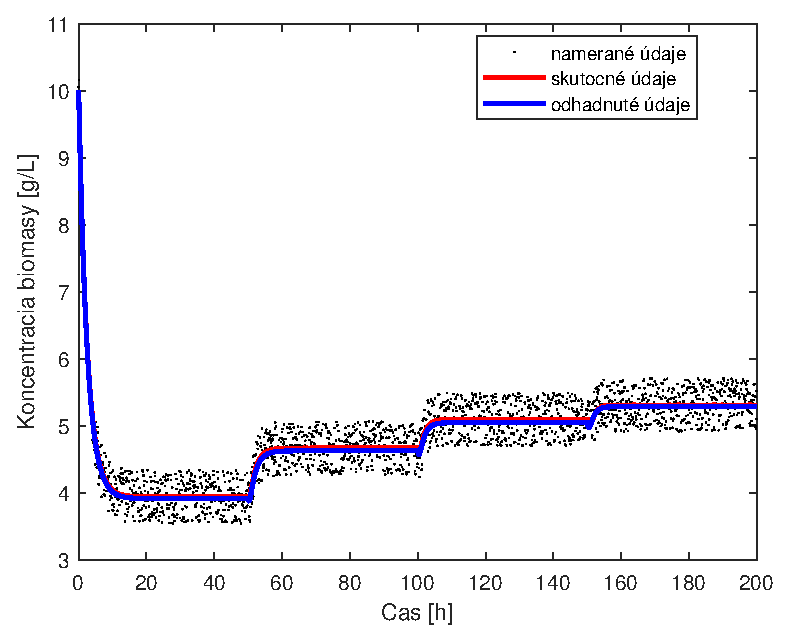
\includegraphics[width=.7\linewidth]{images/der_approximation}
	\caption[]{Časový priebeh koncentrácie biomasy vypočítaný podľa parametrov odhadnutých na základe aproximácie derivácie.}
	\label{fig:8}
\end{figure}

Odhadovať parametre na základe celého modelu je v tomto prípade omnoho efektívnejšie. Vyhneme sa tak spomínaným problémom pri odhade parametrov aproximáciou derivácie. Veľkou výhodou tohto prístupu je, že rozptyl šumu môže byť výrazne väčší. Výsledok takéhoto prístupu k odhadu parametrov môžeme vidieť na Obr. \ref{fig:9}. Z obrázku je očividné, že odhadnutý priebeh je kvalitatívne lepší ako v predchádzajúcom prípade.
% RP: Hm, toto porovnanie nefunguje kedze ste na Obr. 8 neukazali koncentraciu susbstratu. Citatel ma skor pocit, ze ho chcete zavadzat.

\begin{figure}
	\centering
	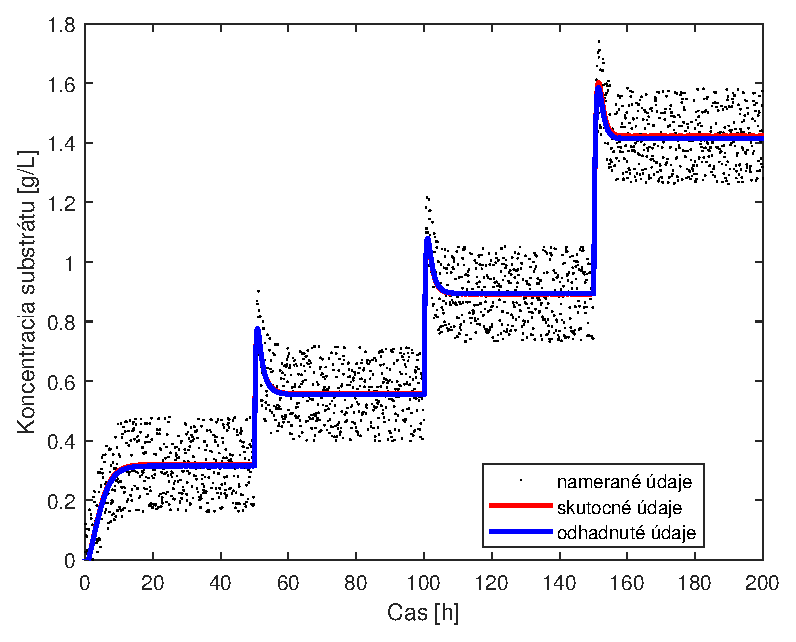
\includegraphics[width=.7\linewidth]{images/param_approx_diff_eq}
	\caption[]{Časový priebeh koncentrácie substrátu vypočítaný podľa parametrov odhadnutých na základe diferenciálnych rovníc modelu a nameranej koncentrácie substrátu.}
	\label{fig:9}
\end{figure}

Výsledky porovnania optimalizačných metód pri odhade parametrov na základe modelu a nameranej koncentrácie substrátu sú uvedené v Tabuľke \ref{tab: 4}. Simplexová metóda bola v každom bode efektívnejšia ako metóda Luus--Jaakola. Rozdiel pri týchto metódach je ten, že zatiaľ čo metóda Luus--Jaakola je čisto stochastická metóda, ktorá náhodne umiestňuje body, v ktorých vyhodnocuje účelovú funkciu a porovnáva ju z predchádzajúcimi bodmi, simplexová metóda funguje na aproximácií gradientu a pohybuje sa teda tou najrýchlejšou možnou cestou.
% RP: Simplexova metoda gradient priamo neaproximuje. Dalo by sa skor povedat nieco ako, ze svoj dalsi postup voli na zaklade predoslych hodnot ucelovej funckie. Najrychlejsia mozna by zrejme bola Newtonova metoda, ale ta by si vyzadovali vypocitanie (to nie je uplne jednoduche) alebo aproximaciu gradientu a dokonca aj Hessianu.
Ako už bolo spomínané, tento prístup k odhadu je výpočtovo veľmi náročný, keďže je nutné numericky vyhodnocovať priebeh modelu v každom bode. Tým pádom každé jedno vyhodnotenie účelovej funkcie zaberie značné množstvo času. Ani jedna z týchto metód však nevedie ku globálnemu optimu, ale sú založené na tolerancii nepresnosti.
% RP: V skutocnosti sa aj globalne optimum da najst iba s nejakou odchylkou. ``tolerancia nepresnosti'' je zvlastny vyraz.
Z tohto dôvodu by sme dokázali odhadnúť parametre modelu presnejšie, ak by sme znížili toleranciu nepresnosti.

\begin{table}
	\centering
	\caption{Porovnanie optimalizačných metód pri odhade parametrov modelu biochemického reaktora. Skutočné hodnoty boli: maximálna špecifická rýchlosť rastu $\mu_{m} = $ 0.954 \unitfrac{1}{\hour} a Michaelisova konštanta $K_{M} = $ 1.2 \unitfrac{\gram}{\liter}.}
	\label{tab: 4}
	\begin{tabular}{lll}
		\hline
		& \textbf{Nelder--Mead} & \textbf{Luus--Jaakola} \\
		\hline
		$\mu_{m}$ [\unitfrac{1}{\hour}] & 0.8772 & 1.0500 \\
		$K_{M}$ [\unitfrac{\gram}{\liter}] & 1.0667 & 1.5082 \\
		Počet iterácií & 52 & 349 \\
		Počet vyhodnotení účelovej funkcie & 99 & 698 \\
		Čas [\second] & 4.0351 & 75.0524 \\
		\hline
	\end{tabular}
\end{table}

Zvyšné nepresnosti
% RP: Ake nepresnosti? Ved ten model celkom sedi?
boli spôsobené voľbou nesprávnej štruktúry nášho odhadovaného modelu.
% RP: Volbu nespravnej struktury treba opisat lepsie. Teraz to znie ako by ste niekde urobili chybu. Mali by ste popisat, ze cielom Vasho simulacneho experimentu je ako dopadne odhad parametrov ak by sme zvolili nevhodnu strukturu modelu. Na pocudovanie to dopadne velmi dobre a toto je samozrejme dost rizikove lebo ak model strukturne nesedi (napr. by tam boli nejake skryte/nenajdene nuly) tak sa lahko stane, ze navrhnuty regulator alebo optimalizator setpointu privedie reaktor do stavu vymytia
Žiaľ, tieto informácie nedokážeme získať z nameraných údajov a treba tento problém vyriešiť iným spôsobom. Ako bolo ukázané v článku \cite{HERNANDEZ201946}, jedným z riešení môžu byť hybridné modely. Hybridné modely sú také modely, ktoré majú základ v mechanických modeloch a tieto sú doplnené dátovými modelmi. Dátové modely v tomto prípade úpravujú odchýlky od skutočného modelu, ktoré sa iteratívne aktualizujú na základe informácii zo zariadenia (skutočného modelu). Základnou myšlienkou je vynútiť prispôsobenie podmienok optimality medzi zariadením a rozšíreným modelom pomocou podmienok lineárnej korekcie.
